 \documentclass{article}
\usepackage{setspace}
\usepackage[hidelinks]{hyperref}
\usepackage{url}
\usepackage[utf8]{inputenc}
\usepackage[english]{babel}
\usepackage[a4paper,top=3cm,bottom=2cm,left=3cm,right=3cm,marginparwidth=1.75cm]{geometry}
\usepackage[T1]{fontenc}
\usepackage{graphicx}
\usepackage{longtable} %
\usepackage[caption = false]{subfig}
\usepackage{amsmath}
\usepackage{float}
%\usepackage[style=authoryear,backend=biber]{biblatex}
\usepackage{lineno}
\bibliographystyle{agsm}
\usepackage{natbib}
\usepackage{csquotes}% Recommended
\doublespacing
\newcommand{\HRule}{\rule{\linewidth}{1mm}}
%\addbibresource{references.bib}% Syntax for version >= 1.2
%\bibliography{references.bib}
%
\begin{document}
% title
\title{Functional Response Models and Consumer Temperature}%
\author{Ruth Keane}
\begin{titlepage}

\includegraphics[width=8cm]{logo.eps}\\[1cm] 
\center 
\textsc{\LARGE CMEE Miniproject}\\[1.5cm] 
\textsc{\Large Imperial College London}\\[0.5cm]
\textsc{\large Life Sciences}\\[0.5cm] 
\makeatletter
\HRule \\[0.4cm]
{ \huge \bfseries \@title}\\[0.4cm] % Title of your document
\HRule \\[1.5cm]
\makeatother
\Large \emph{Author:}\\
Ruth Keane \\[3cm] % Your name
\input{../Results/Tables/wordcount.txt}\\
{\large \today}\\[2cm] % Date, change the \today to a set date if you want to be precise
\vfill % Fill the rest of the page with whitespace
\clearpage
\end{titlepage}
\linenumbers
\begin{abstract}
this is the abstract.
\end{abstract}
\section{Introduction}
\subsection{Functional Responses and existing models}
The functional response describes how predators respond to changes in prey density \cite{hollingsawfly1959,Solomon1949}. As prey numbers increase, the consumption rate of predators initially increases then levels out, however the specific shape of the period of increase can vary \cite{hollingsawfly1959}. Holling modelled the functional response and suggested three different forms which worked for different types of organisms \cite{hollingsawfly1959}. These are Type I, where the rate of increase in prey consumption with prey density is constant before the plateau, type II where the rate of increase in prey consumption with prey density is decreasing (i.e the curve is hyperbolic %jesche 2002
and type III, where the  rate of increase in prey consumption with prey density increases then decreases \cite{hollingsawfly1959}. The type I model can be described by equation \ref{type1}, the type II model can be described by equation \ref{type3} where $x_R$ is the resource density, $c$ is the number of prey consumed per predator per unit time,$a$ is the discovery or search rate of the consumer and $h$ is the handling time \cite{Dawes2013,Holling1959}. The type III model can be described by a generalised version of equation \ref{type2}, equation \ref{type3} where $q$ changes the shape of the curve \cite{Dawes2013}. %explain how - dawes? or unnecessary
When $q=0$, the model is type II and when $q>0$,the model is type III \cite{Dawes2013}. These equations are often written with $Y$, the number of prey consumed per predator, instead of $c$ and $T$, the time, on the right side of the equation, however these equations are equivalent as $c=\frac{Y}{T}$.%is this line helping?
\begin{equation}\label{type1}
    c=ax_R
\end{equation}
\begin{equation}\label{type2}
c=\frac{ax_R}{1+hax_R}
\end{equation}
\begin{equation}\label{type3}
c=\frac{ax_R^{q+1}}{1+hax_R^{q+1}}
\end{equation}

It is important to note that both the search rate and handling times are functions of different aspects of attacking and eating prey \cite{Hassel1976TheDeath-Rate}. %best once synced/. 
In general, the Holling type II model is very successful, especially considering its simplicity however there are examples where data is better described by a more complex model, such as a type III Holling model \cite{Hassel1976TheDeath-Rate} . 
Many other models exist to describe the functional response, often based on variations of the Holling equation accounting for different behavioural aspects  \cite{Jeschke2002PredatorPrey}. \cite{Jeschke2002PredatorPrey} attempted to separate handling and digestion time from  $h$. In this example, the model curve tends to be similar to the Holling type II functional response curve, but is more flexible and when both handling time and digestion time are high, the curve is quite different. 
In addition, if values of $a$ or $h$ change with prey density, then the Holling II model may not fit well  (as $a$ and $h$ are constant in this model). In these examples, the type III Holling model can be a good model \cite{Hassel1976TheDeath-Rate}. 
%+eg? 
\subsection{Temperature and Functional Responses}

\subsection{Models}
Models can be phenomenological or mechanistic. In mechanistic models, all parameters have biological meaning and in phenomenological models they do not, instead a function is used that fits the data or processes %otto day ref  
emodels are  %see becker paper and textbppl
Phenomenological models may fit better to data and can be very useful fin the absence of mechanistic models. They can be easier to understand, however do not have as much biological meaning as mechanistic models. %%
however mechanistic models can improve our understanding of biology and are useful for extrapolating more accurately because when the meanings of parameters of known, biological constraints to be included. %%?%??
The Holling models described above are mechanistic to some extent however the type III model is more phenomenological due to the non-biological parameter $q$. Even the Holling type II model may be partially phenomenological because the values of $a$ and $h$ are a function of , multiple biological components \cite{Hassel1976TheDeath-Rate}.%maybe better in discussion. 


\subsection{This work}
In this paper, 5 models were fitted to experimental functional response data: Holling's type I, Holling's type II, Holling's type III, a polynomial model of degree two (to capture increasing and levelling out of the functional response) and a polynomial model of degree three (to capture a change in the rate of increase of the functional response.Then the best model for each experiment was determined. This was analysed and compared to temperatures. In addition the parameters of the Holling's models were compared to the consumer temperature.\\
It was expected that the Holling type III model would be able to fit better to the data but may have a higher AIC value due the the extra parameter. %TEMPERATURE EXPECTATIONS
%
\section{Methods}
\subsection{Computing Tools}
Bash was used to compile the pdf of the tex file, to calculate and format the word count of the project, using teXcount and to run the project files. This was used due to the ease off accessing files and files contents compared to other languages as well as its ability to run python and R scripts.
Python was used to initially sort the data, add new columns to the dataset and remove datasets with an insufficient number of points and export this updated dataframe as a csv. These tasks are well suited to Python's abilities.
R was used to model to data, plot graphs and analyse the data. This is due to R's dataframe structures which make it very easy to store and manipulate variables. In addition ggplot2's plotting is very flexible.
%what packages were used and why
\subsection{Initial Data Sorting}
The data used was from the Biotraits database \cite{Dell2013}, which contains information collated from different studies about how biological traits respond to environmental drivers. The parameters of interest here were the number of prey the predator consumed per unit time and the resource density. Data sorting was carried out in python version 2.7. New columns were added and experiments with less than six experiments were removed. This new dataset was exported to a csv for model fitting. The
\subsection{Model Fitting}
The data were fitted to five different models, a quadratic model, a cubic model and the three Holling models \cite{Holling1959} using R 3.6.2 \cite{RCoreTeam2017}. The Holling models were the type I model (equation \ref{type1}, a linear model where the intercept was the origin), type II model (equation \ref{type2}) and generalised type III model (equation \ref{type3}).
Models were fitted sequentially for each experiment and plotted. This allowed the fit to be visually inspected as the model fitting process was improved.
\subsubsection{Linear models}
 The Holling type I, quadratic and cubic models models were fitted using lm (base R). For the quadratic and cubic models, poly was used to compute orthogonal polynomials to avoid correlation of variables.
\subsubsection{Non-linear Models}
The Holling type II and type III models were fitted using NLSlm (from the package minpack.lm \cite{Elzhov2016}). The coefficients $a$, $h$, and $q$ were given a lower bound of zero and the maximum number of iterations was set to $1000$. For both type II and type III models, starting values were calculated using starting value functions where $a$, $h$ and $q$ were estimated, followed by sampling positive values around these initial values and repeatedly running the models and storing the coefficients and AIC values of these models. The coefficients of the model with the lowest AIC were used as the initial values for the main model fitting step. The initial value for $h$ was the maximum value of $c$. The initial value for $a$ was the initial steep part of the curve which was calculated by repeatedly fitting linear models the dataset then deleting the maximum value of $x_R$ and storing the largest gradient of these models.For the type III model, this initial value of $q$ was set at %pick and also justify
Once the starting values had been determined, the models were rerun with these initial values and plotted (with the other models). %try?
\subsection{Data Analysis}
%how many 
Data analysis was carried out in R 3.6.2\cite{RCoreTeam2017}.The models were compared using AIC and the most appropriate model was determined for each dataset. AIC was used because other techniques to compare models are not appropriate for non linear models.\\  %why AIC not bic
The confidence intervals for values of $q$ were calculated and (using two times the standard error). When the confidence interval for $q$ overlapped zero, the best AIC was recalculated for the remaining Holling models (because when the confidence interval for $q$ is zero, the type III model is the same as the type III model.  %%remove this?
A chi-square ($\chi^2$) goodness of fit test was carried out on the best model and the best model type (phenomenological or mechanistic) to determine if the number of models in each category was significantly different.\\
The p-value of each parameter was stored and if the model was not significant, the parameter was removed from analysis of that parameter. Shapiro-Wilk tests were used to test the log consumer temperatures and log parameter values and found that they were not normally distributed. In addition, there were ties in the data so Spearman's rank correlation could not be calculated.  Kendall rank order correlation tests were carried out on consumer temperatures and log search rate and consumer temperatures and log handling time for each of the Holling models. Log of the parameters was used because both search rate and the handling time values were mostly very low with  a few very large values. The search rate for type III models could not be tested due to a low number of models were search rate was significant. \\ 
A chi-square ($\chi^2$) test carried out on resource temperature and best model. The temperature values were discretised by creating an expectation table with intervals of five degrees and combining these intervals until the expected values were all greater than five.
%talk about stats stuff- tests 
\section{Results}
%figs will need to be saved into code directory probs
\subsection{Number of Fits}
Many of the models fit well to the data, for example (Figure\ref{fig:2}). Most models successfully fit the data. Of the 241 datasets, only $\input{../Results/Tables/failII}$ Holling type II models and $\input{../Results/Tables/failIII}$ Holling type II models did not converge.  % don't love format for this , where should this go!
\begin{figure}[h!] %h forces it to be at this location
    \centering
    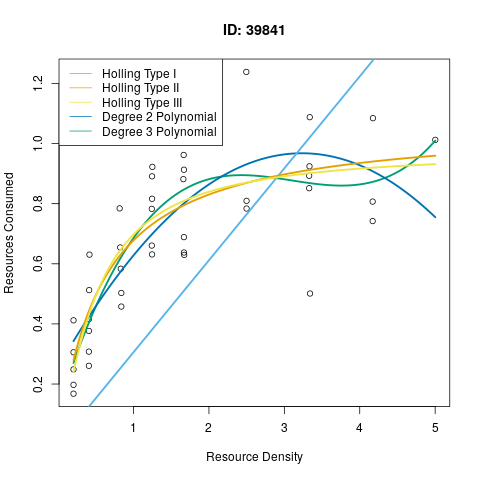
\includegraphics[width=4in]{../Results/Plots/39841.png}
    \caption{This is a graph for the experiment with ID 39841}
    \label{fig:2}
\end{figure}
%best model, significance
\subsection{Best Model}
The Holling's type II model was most frequently the best model ($\input{../Results/Tables/holIIbest}\%$) and the polynomial of degree 2 was most frequently the second best model ($\input{../Results/Tables/poly32best}\%$) (Figure \ref{fig:bestmodel}).
The mechanistic models were marginally more often the best model ($\%$)than the mechanistic models (Figure \ref{fig:modelbesttype} )
\begin{figure}[h!]
\centering
\subfloat[Number of times that each model was the best model]{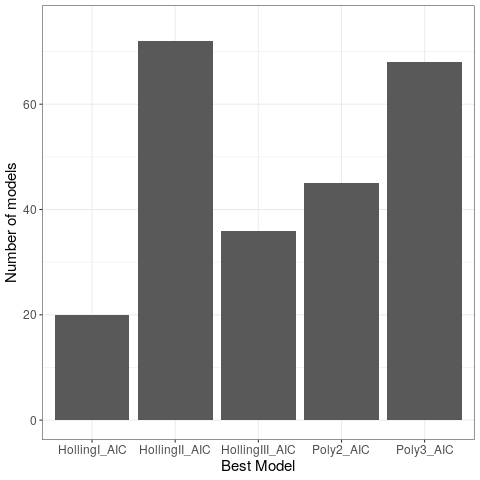
\includegraphics[width = 3in]{../Results/Plots/modelbest.png}}
\subfloat[Number of times that each model was the second best model]{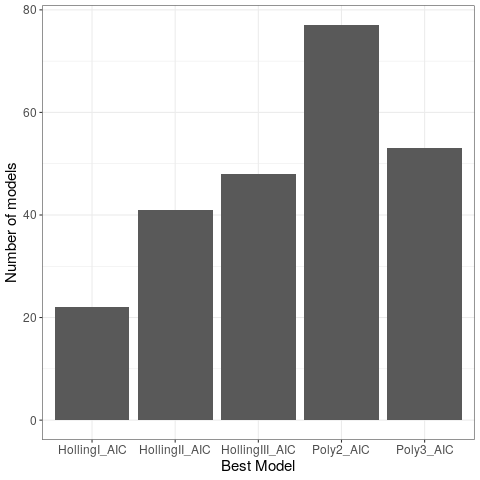
\includegraphics[width = 3in]{../Results/Plots/modelsecondbest.png}}
\caption{Best and second best model from the lowest and second lowest AIC values. Models are Holling type I, Holling type II, Holling type II, polynomial of degree 2, polynomial of degree 3. $n=241$}
\label{fig:bestmodel}
\end{figure}
\begin{figure}[h!] %h forces it to be at this location
    \centering
    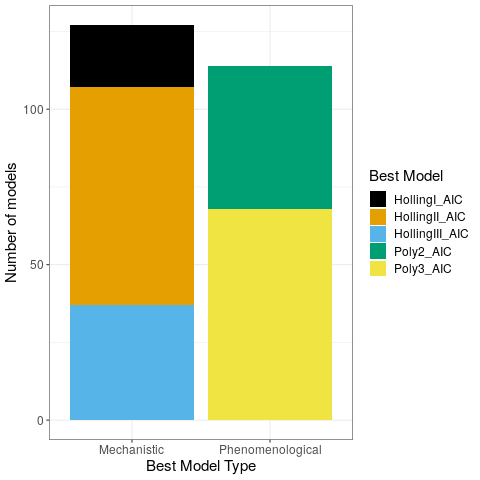
\includegraphics[width=3in]{../Results/Plots/modelbesttype.png}
    \caption{Number of models where the best type was phenomenological or mechanistic. Colour is the model. $n=241$}
    \label{fig:modelbesttype}
\end{figure}
The distribution of the best model was not best described by a uniform distribution ($p<0.01$) but the distribution of the best model type was (p<0.05) (Table\ref{chitable}),
\input{../Results/Tables/output_chitable_latex.txt}
\subsection{Best Holling Model}
Of the three Holling models, the type II model was the best (Figure\ref{fig:bestholandrecalmodel}).The best Holling model was recalculated, removing the type III Holling model when the confidence interval for $q$ spanned $0$. This affected $\input{../Results/Tables/recaldiff}$ models. The majority of these were best described by the Holling type II model of the other Holling models, but some were better described by the type I model (Figure \ref{fig:bestholandrecalmodel}) %discussion- it was expected that would make just holling 2 larger,
\begin{figure}[h!]
\centering
\subfloat[Number of times that each model was the best  Holling model]{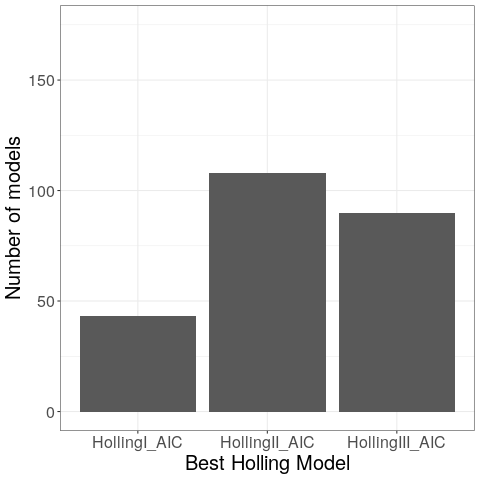
\includegraphics[width = 3in]{../Results/Plots/modelbestholl.png}}
\subfloat[Number of times that each model was the best Holling model, when the best Holling model was recalculated if the confidence intervals of $q$ spanned $0$]{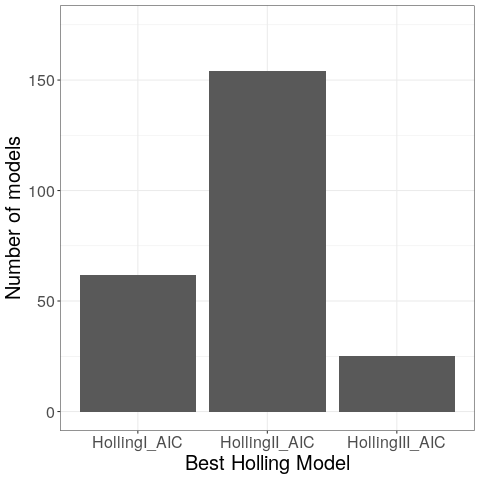
\includegraphics[width = 3in]{../Results/Plots/modelbesthollrecal.png}}
\caption{Best model from the lowest AIC values (of the Holling model). Models are Holling type I, Holling type II and Holling type II. $n=241$}
\label{fig:bestholandrecalmodel}
\end{figure}
\subsection{Temperature and Best Model}
For the most part, the shape of the distribution of the best model was the same at different temperatures however the at $20-25$ degree interval the polynomial of degree was a lot more successful than the  Holling II model (Figure \ref{fig:tempmodel}). The consumer temperature did not significantly effect which model fit the data the best ($\chi^2=\input{../Results/Tables/chitemp}$,$p=\input{../Results/Tables/ptemp}$,$df=12$). 
\begin{figure}[h!] %h forces it to be at this location
    \centering
    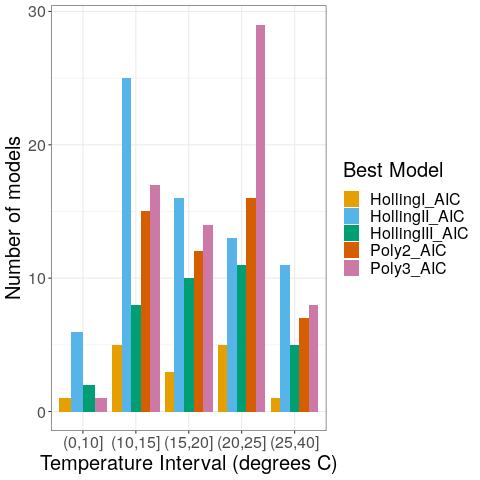
\includegraphics[width=3.5in]{../Results/Plots/tempmodel.png}
    \caption{Number of times that each model was the best model at each consumer temperature interval. Colour is the best model. $n=241$}
    \label{fig:tempmodel}
\end{figure}
\subsection{Temperature and Parameter Values}
The handling time was and the search rate was
The consumer temperatures are associated with the search rate for type I and type II Holling models and handling time for type II and type III Holling models.(Figure \ref{fig:tempparam},Table \ref{Paramtemp}). % stats
\input{../Results/Tables/output_temp_con_latex.txt}
The search rate is smaller and less varied at intermediate temperatures, however at very low and very high temperatures, the temperature is very varied and can be very high. There is a weak negative correlation. The handling time shows a weak positive correlation with consumer temperature.
%stats
\begin{figure}[h!t]
\centering
\subfloat[Consumer temperature and log search rate for type I Holling model]{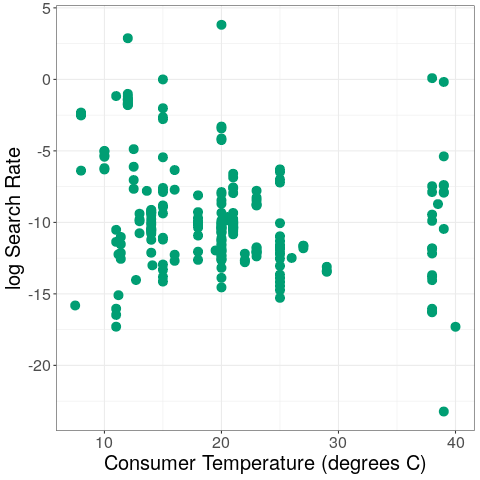
\includegraphics[width = 2.5in]{../Results/Plots/plot1conA.png}}\\
\subfloat[Consumer temperature with log search rate for type II Holling model]{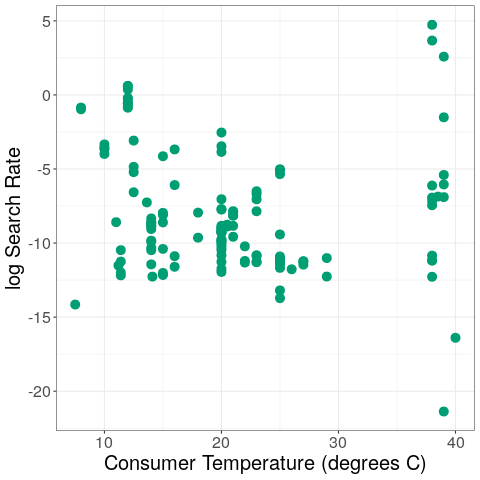
\includegraphics[width = 2.5in]{../Results/Plots/plot2conA.png}}
\subfloat[Consumer temperature with log handling time for type II Holling model]{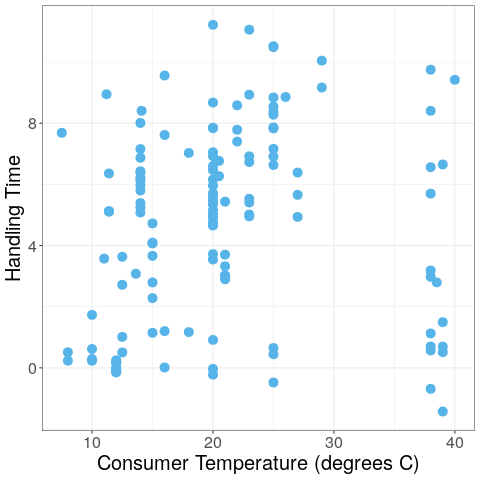
\includegraphics[width = 2.5in]{../Results/Plots/plot2conH.png}} \\
\subfloat[Resource temperature with log search rate for type III Holling model]{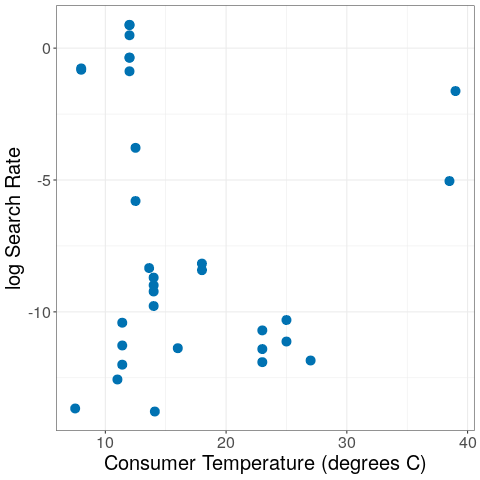
\includegraphics[width = 2.5in]{../Results/Plots/plot3conA.png}}
\subfloat[Consumer temperature with log handling time for type III Holling model]{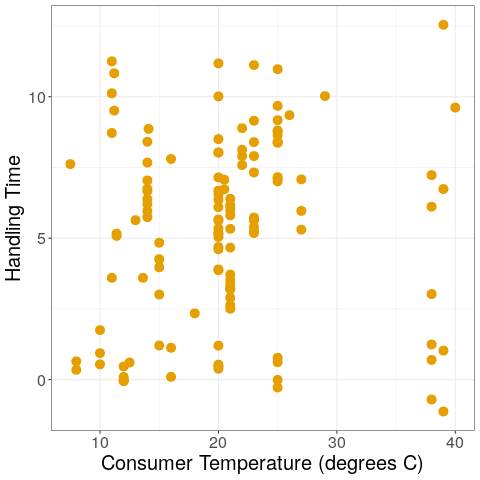
\includegraphics[width = 2.5in]{../Results/Plots/plot3conH.png}}
\caption{Logged parameter values and Consumer temperature for Type I, Type II and Type II Holling Models.}
\label{fig:tempparam}
\end{figure}
\section{Discussion}
%go through each model and talk about how well it fit 
%significance? 
\section{Conclusion}
%answer question


%\begin{enumerate}
%\item A citation command in parentheses: \cite{hollingsawfly1959}.
%\item A citation command for use in the flow of text: As \textcite{Holling1966} said \dots
%\item A citation command which automatically switches style depending on location and the option setting in the package declaration (see line 12 in the LaTeX source code). In this case, it produces a citation in parentheses: \autocite{hollingsawfly1959}.
%\end{enumerate}


\clearpage{}

\bibliography{main.bib}
%\bibliographystyle{plain}

\end{document}

